\begin{frame}{El Desafío de las Altas Temperaturas}
  \frametitle{Requerimientos Térmicos en la Nueva Siderurgia}
  El desarrollo industrial impuso condiciones operativas que excedían la
  capacidad de los materiales convencionales.

  \begin{columns}[T]
    \begin{column}{0.6\textwidth}
      \begin{itemize}[<+->]
        \item La producción de \textbf{acero} a escala industrial y la
          optimización de \textbf{máquinas de vapor} requerían hornos y calderas
          que operaran a temperaturas sostenidas y elevadas.
        \item Los materiales de construcción existentes, como ladrillos comunes
          y mampostería, sufrían fallas estructurales y fusión bajo estas
          condiciones.
      \end{itemize}
    \end{column}
    \begin{column}{0.4\textwidth}
      \begin{figure}
        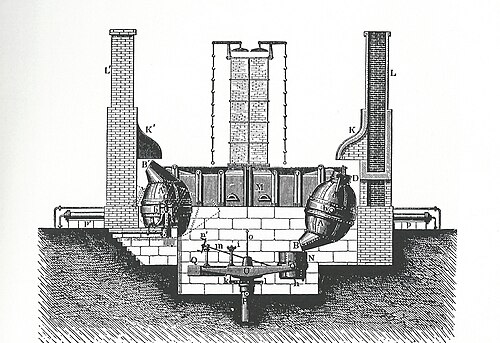
\includegraphics[width=\textwidth]{../figures/bessemer.jpg}
        \caption{Convertidor Bessemer. \cite{wiki:bessemer}}
      \end{figure}
    \end{column}
  \end{columns}
\end{frame}

\begin{frame}{Aplicación de Cerámicos Refractarios}
  \frametitle{Soluciones para la Contención Térmica}
  La solución técnica se basó en el desarrollo de cerámicos especializados.

  \begin{columns}[T]
    \begin{column}{0.6\textwidth}
      \begin{itemize}[<+->]
        \item Se industrializó la producción de ladrillos a partir de
          \textbf{arcillas refractarias (fireclay)} y \textbf{sílice
          (\ce{SiO2})}.
        \item Su función principal fue el revestimiento interno de altos hornos,
          convertidores y calderas.
        \item \textbf{Impacto técnico:} La capacidad de contener energía térmica
          fue un requisito indispensable para la siderurgia moderna.
      \end{itemize}
    \end{column}
    \begin{column}{0.4\textwidth}
      \begin{figure}
        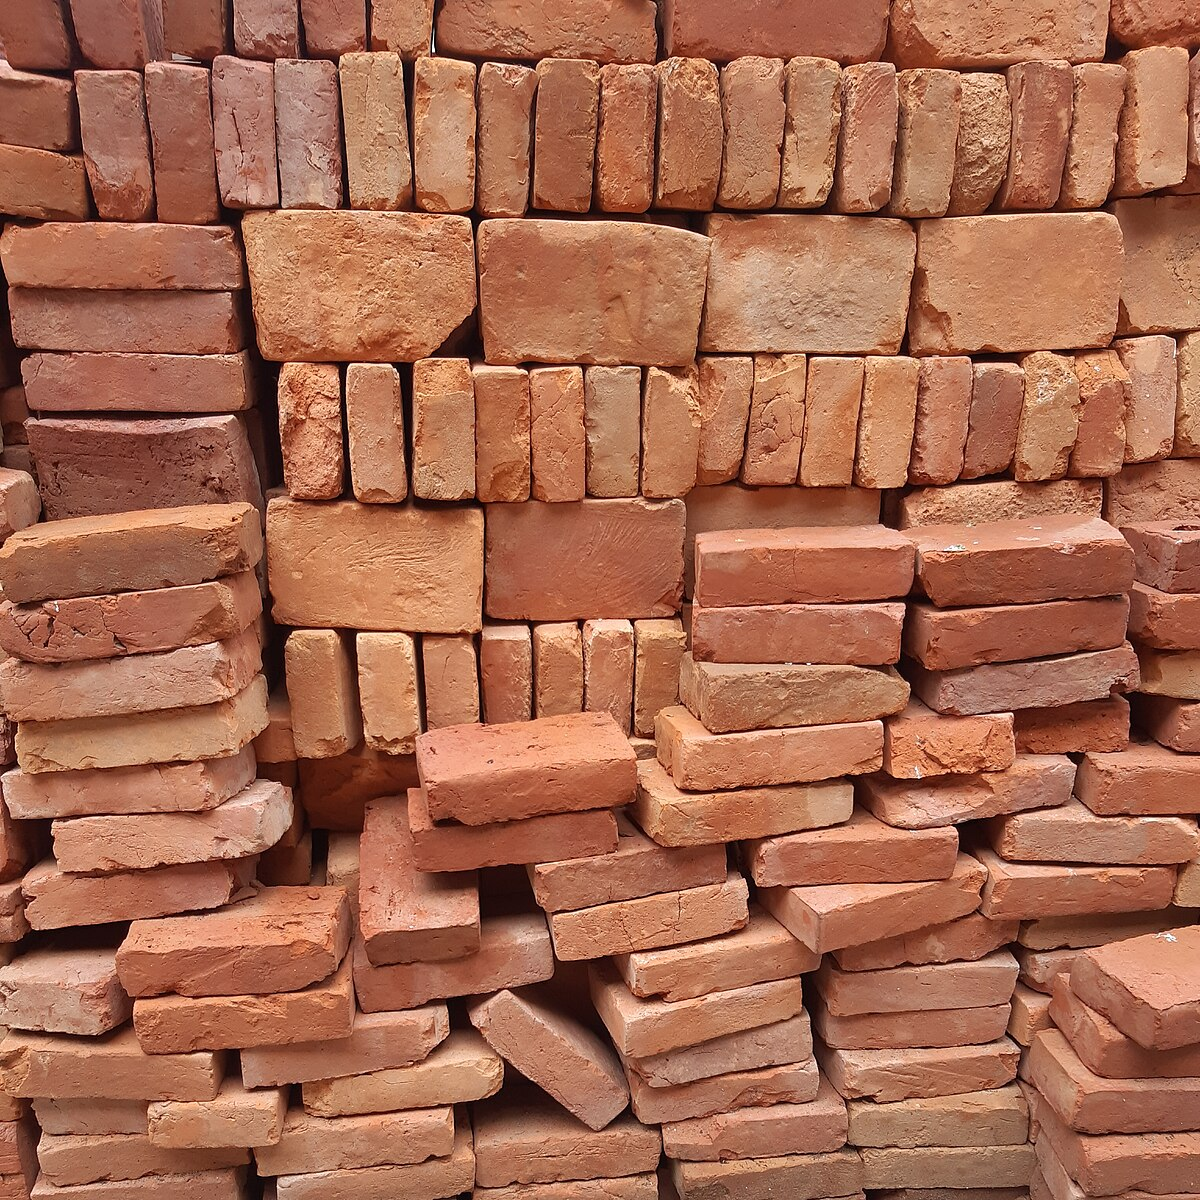
\includegraphics[width=\textwidth]{../figures/refractory_bricks.jpg}
        \caption{Bloques de Ladrillos. \cite{wiki:fired_bricks}}
      \end{figure}
    \end{column}
  \end{columns}
\end{frame}

\begin{frame}{Contención de Agentes Corrosivos}
  La emergente industria química requería recipientes y ductos con alta inercia
  química.

  \begin{columns}[T]
    \begin{column}{0.6\textwidth}
      \begin{itemize}[<+->]
        \item El \textbf{gres cerámico vitrificado} se estableció como el
          material estándar por su baja porosidad y alta resistencia a ácidos.
        \item Se empleó en la fabricación de contenedores y tuberías para la
          producción de ácido sulfúrico.
      \end{itemize}
    \end{column}
    \begin{column}{0.4\textwidth}
      \begin{figure}
        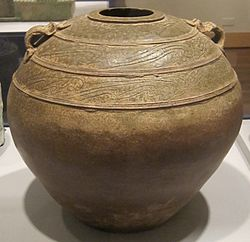
\includegraphics[width=0.8\textwidth]{../figures/stoneware_jars.jpg}
        \caption{Alfarería de Piedra. \cite{wiki:stoneware}}
      \end{figure}
    \end{column}
  \end{columns}
\end{frame}

\begin{frame}{Rol en la Infraestructura Sanitaria}
  \frametitle{Materiales para el Saneamiento Urbano}
  La rápida urbanización demandó soluciones duraderas para la gestión de aguas
  residuales.

  \begin{columns}[T]
    \begin{column}{0.6\textwidth}
      \begin{itemize}[<+->]
        \item La crisis sanitaria en centros industriales impulsó el desarrollo
          de redes de saneamiento a gran escala.
        \item Las \textbf{tuberías de gres vitrificado} ofrecían la durabilidad
          e impermeabilidad necesarias para los primeros sistemas de
          alcantarillado.
      \end{itemize}
    \end{column}
    \begin{column}{0.4\textwidth}
      \begin{figure}
        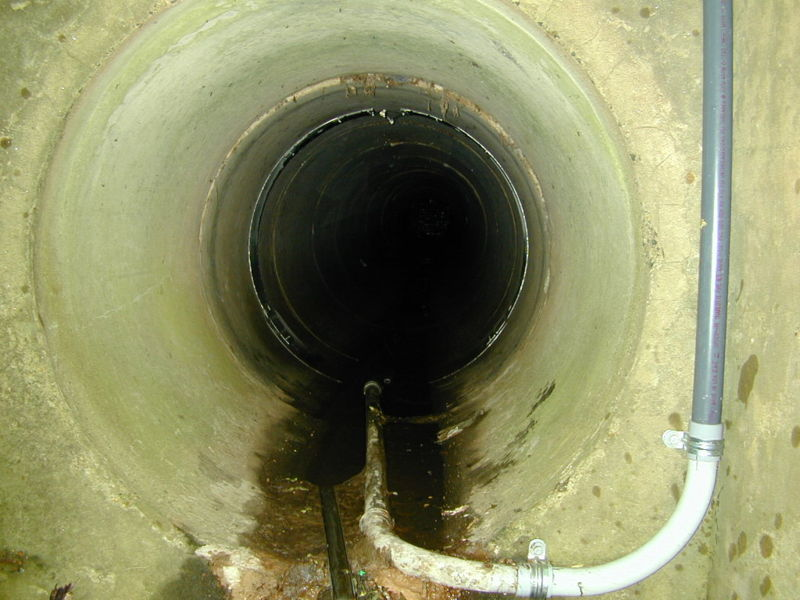
\includegraphics[width=\textwidth]{../figures/sewer_pipes.jpg}
        \caption{Alcantarillas. \cite{wiki:sewer}}
      \end{figure}
    \end{column}
  \end{columns}
\end{frame}

\begin{frame}{El Problema del Aislamiento Eléctrico}
  \frametitle{Requerimientos para la Transmisión de Energía}
  La distribución de energía eléctrica presentaba un desafío fundamental: su
  aislamiento seguro y eficiente.

  \begin{columns}[T]
    \begin{column}{0.6\textwidth}
      \begin{itemize}[<+->]
        \item Se necesitaba un material de \textbf{alta resistividad
          dieléctrica} para prevenir pérdidas de corriente y cortocircuitos.
        \item Dicho material debía poseer \textbf{estabilidad mecánica y
          ambiental} para su uso en exteriores.
      \end{itemize}
    \end{column}
    \begin{column}{0.4\textwidth}
      \begin{figure}
        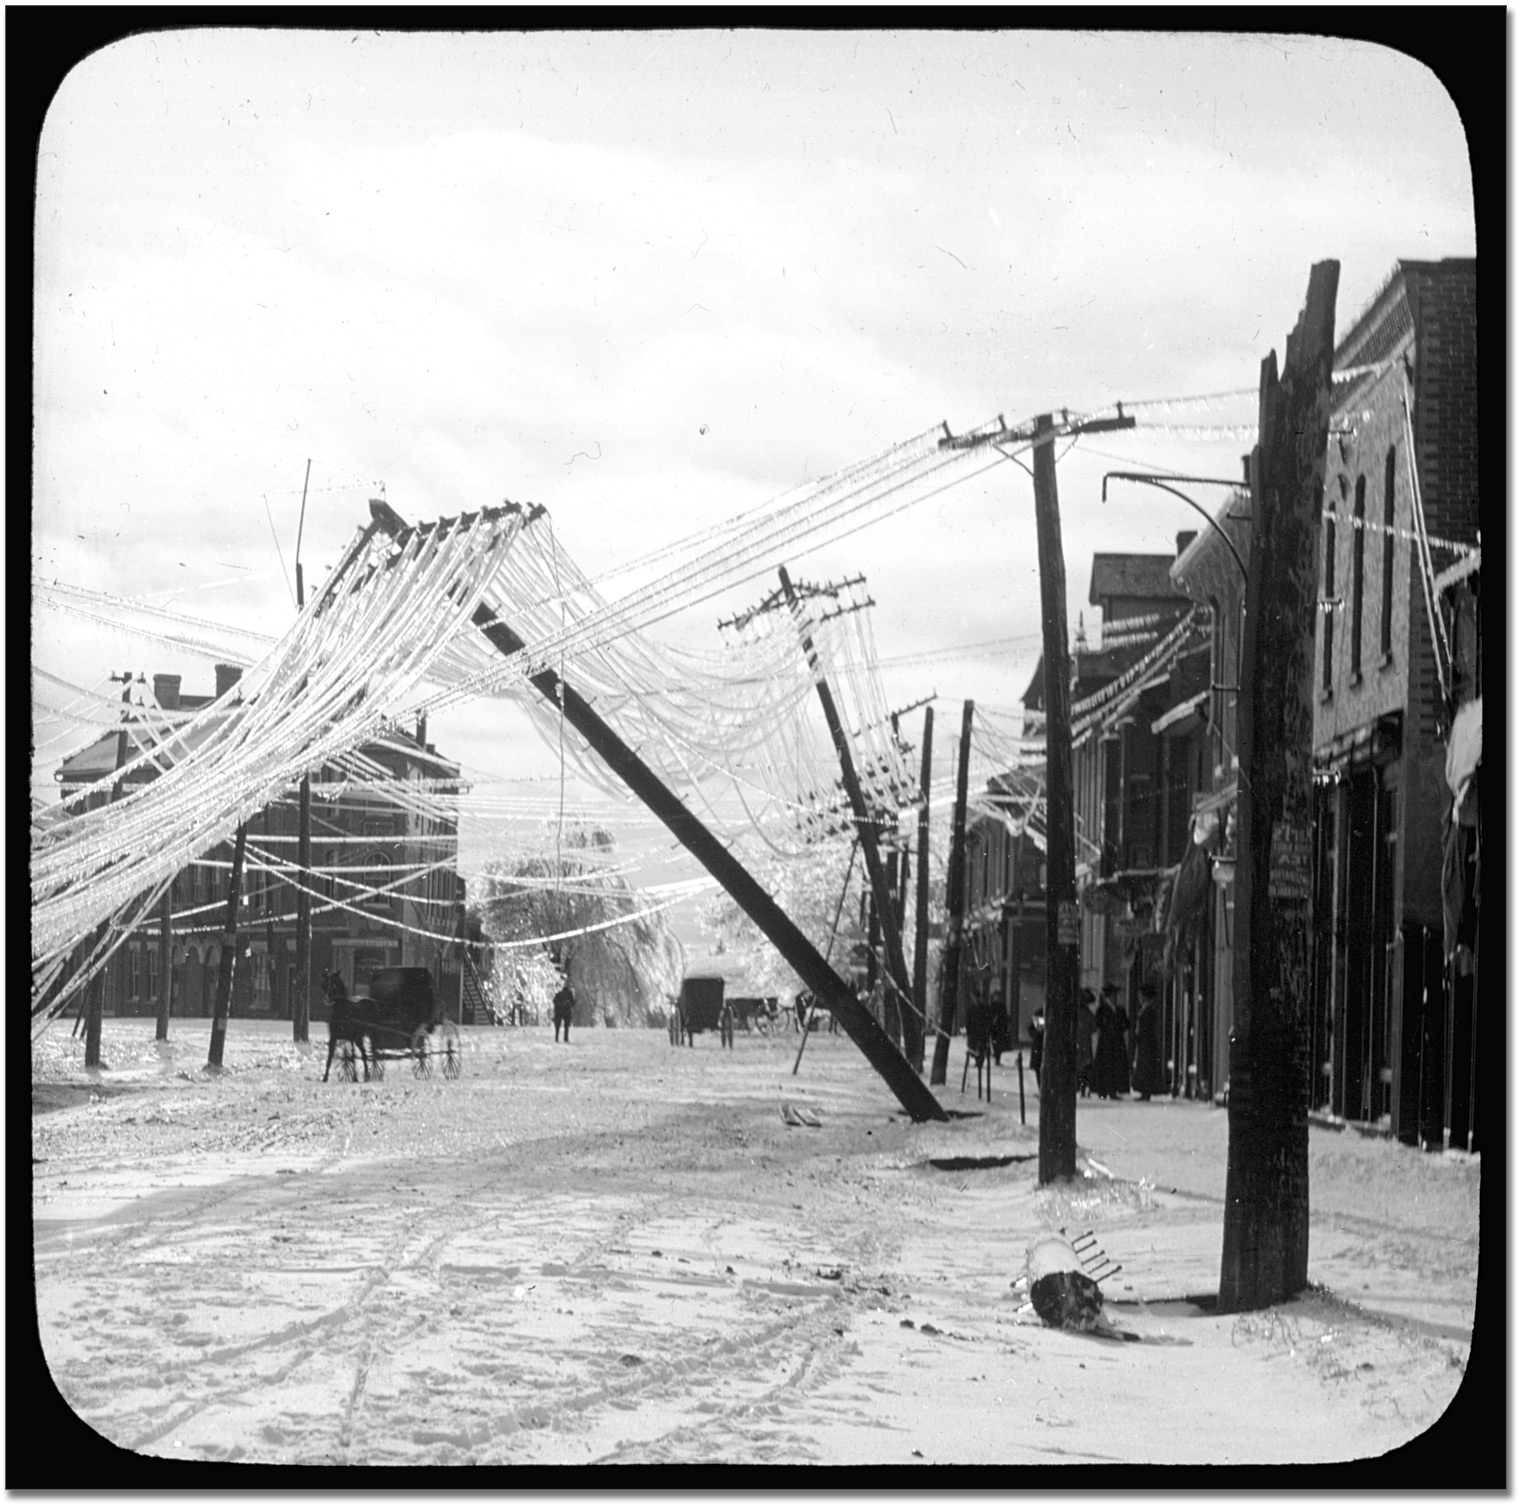
\includegraphics[width=0.8\textwidth]{../figures/early_power_lines.jpg}
        \caption{Tormenta en Ontario. \cite{wiki:ice_storm_photo}}
      \end{figure}
    \end{column}
  \end{columns}
\end{frame}

\begin{frame}{La Porcelana como Aislante Eléctrico}
  \frametitle{Material Dieléctrico Estándar}
  La cerámica, una vez más, proveyó la solución técnica óptima.

  \begin{columns}[T]
    \begin{column}{0.6\textwidth}
      \begin{itemize}[<+->]
        \item La \textbf{porcelana eléctrica}, densa a base de caolín,
          feldespato y cuarzo, demostró tener propiedades dieléctricas y
          mecánicas superiores.
        \item Su principal aplicación fue la fabricación en masa de
          \textbf{aisladores} para las redes de telegrafía, telefonía y
          transmisión de energía.
      \end{itemize}
    \end{column}
    \begin{column}{0.4\textwidth}
      \begin{figure}
        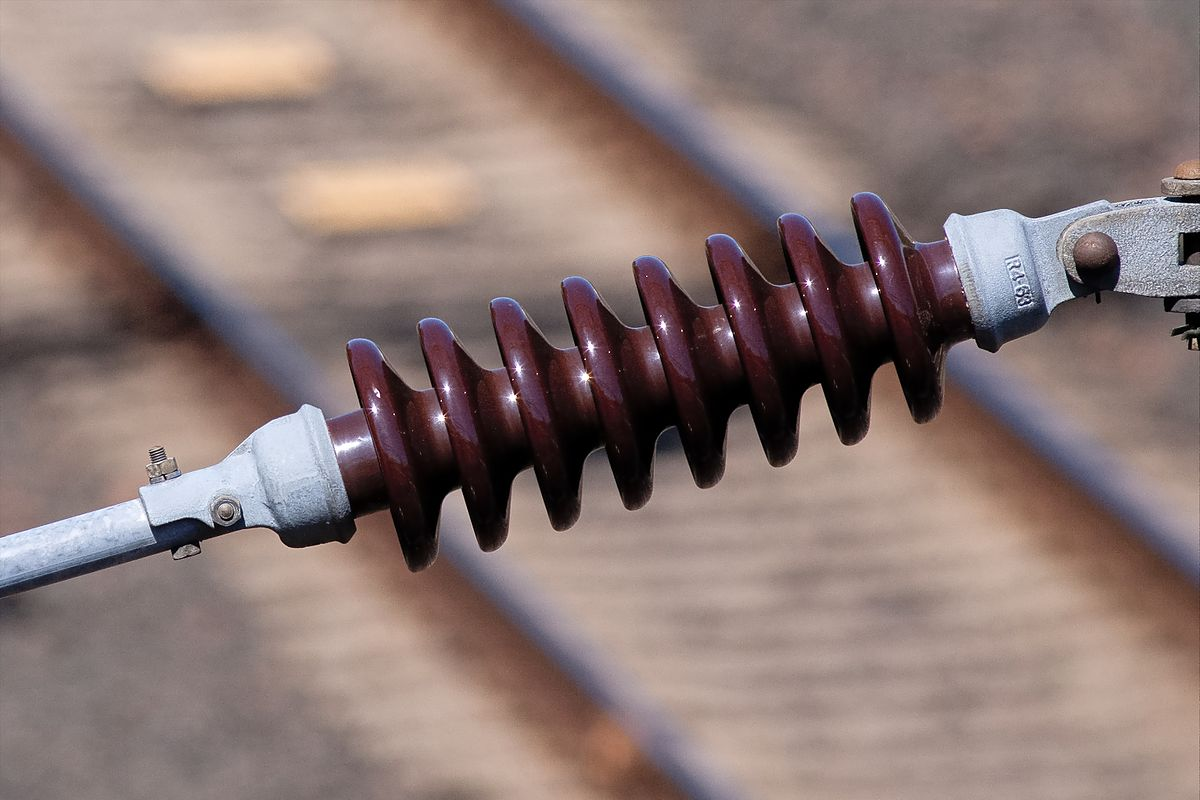
\includegraphics[width=\textwidth]{../figures/porcelain_insulators.jpg}
        \caption{Aislantes cerámicos. \cite{wiki:insulator}}
      \end{figure}
    \end{column}
  \end{columns}
\end{frame}

\begin{frame}{Nuevos Requerimientos para la Electrónica}
  \frametitle{El Advenimiento de los Circuitos Eléctricos}
  El desarrollo de la radio y la telegrafía sin hilos introdujo nuevos
  requerimientos a nivel de componente.

  \begin{columns}[T]
    \begin{column}{0.6\textwidth}
      \begin{itemize}[<+->]
        \item Los componentes electrónicos requerían materiales que ofrecieran
          \textbf{aislamiento eléctrico a pequeña escala}.
        \item Adicionalmente, era necesaria una alta \textbf{estabilidad
          dimensional y térmica} para garantizar el funcionamiento fiable.
      \end{itemize}
    \end{column}
    \begin{column}{0.4\textwidth}
      \begin{figure}
        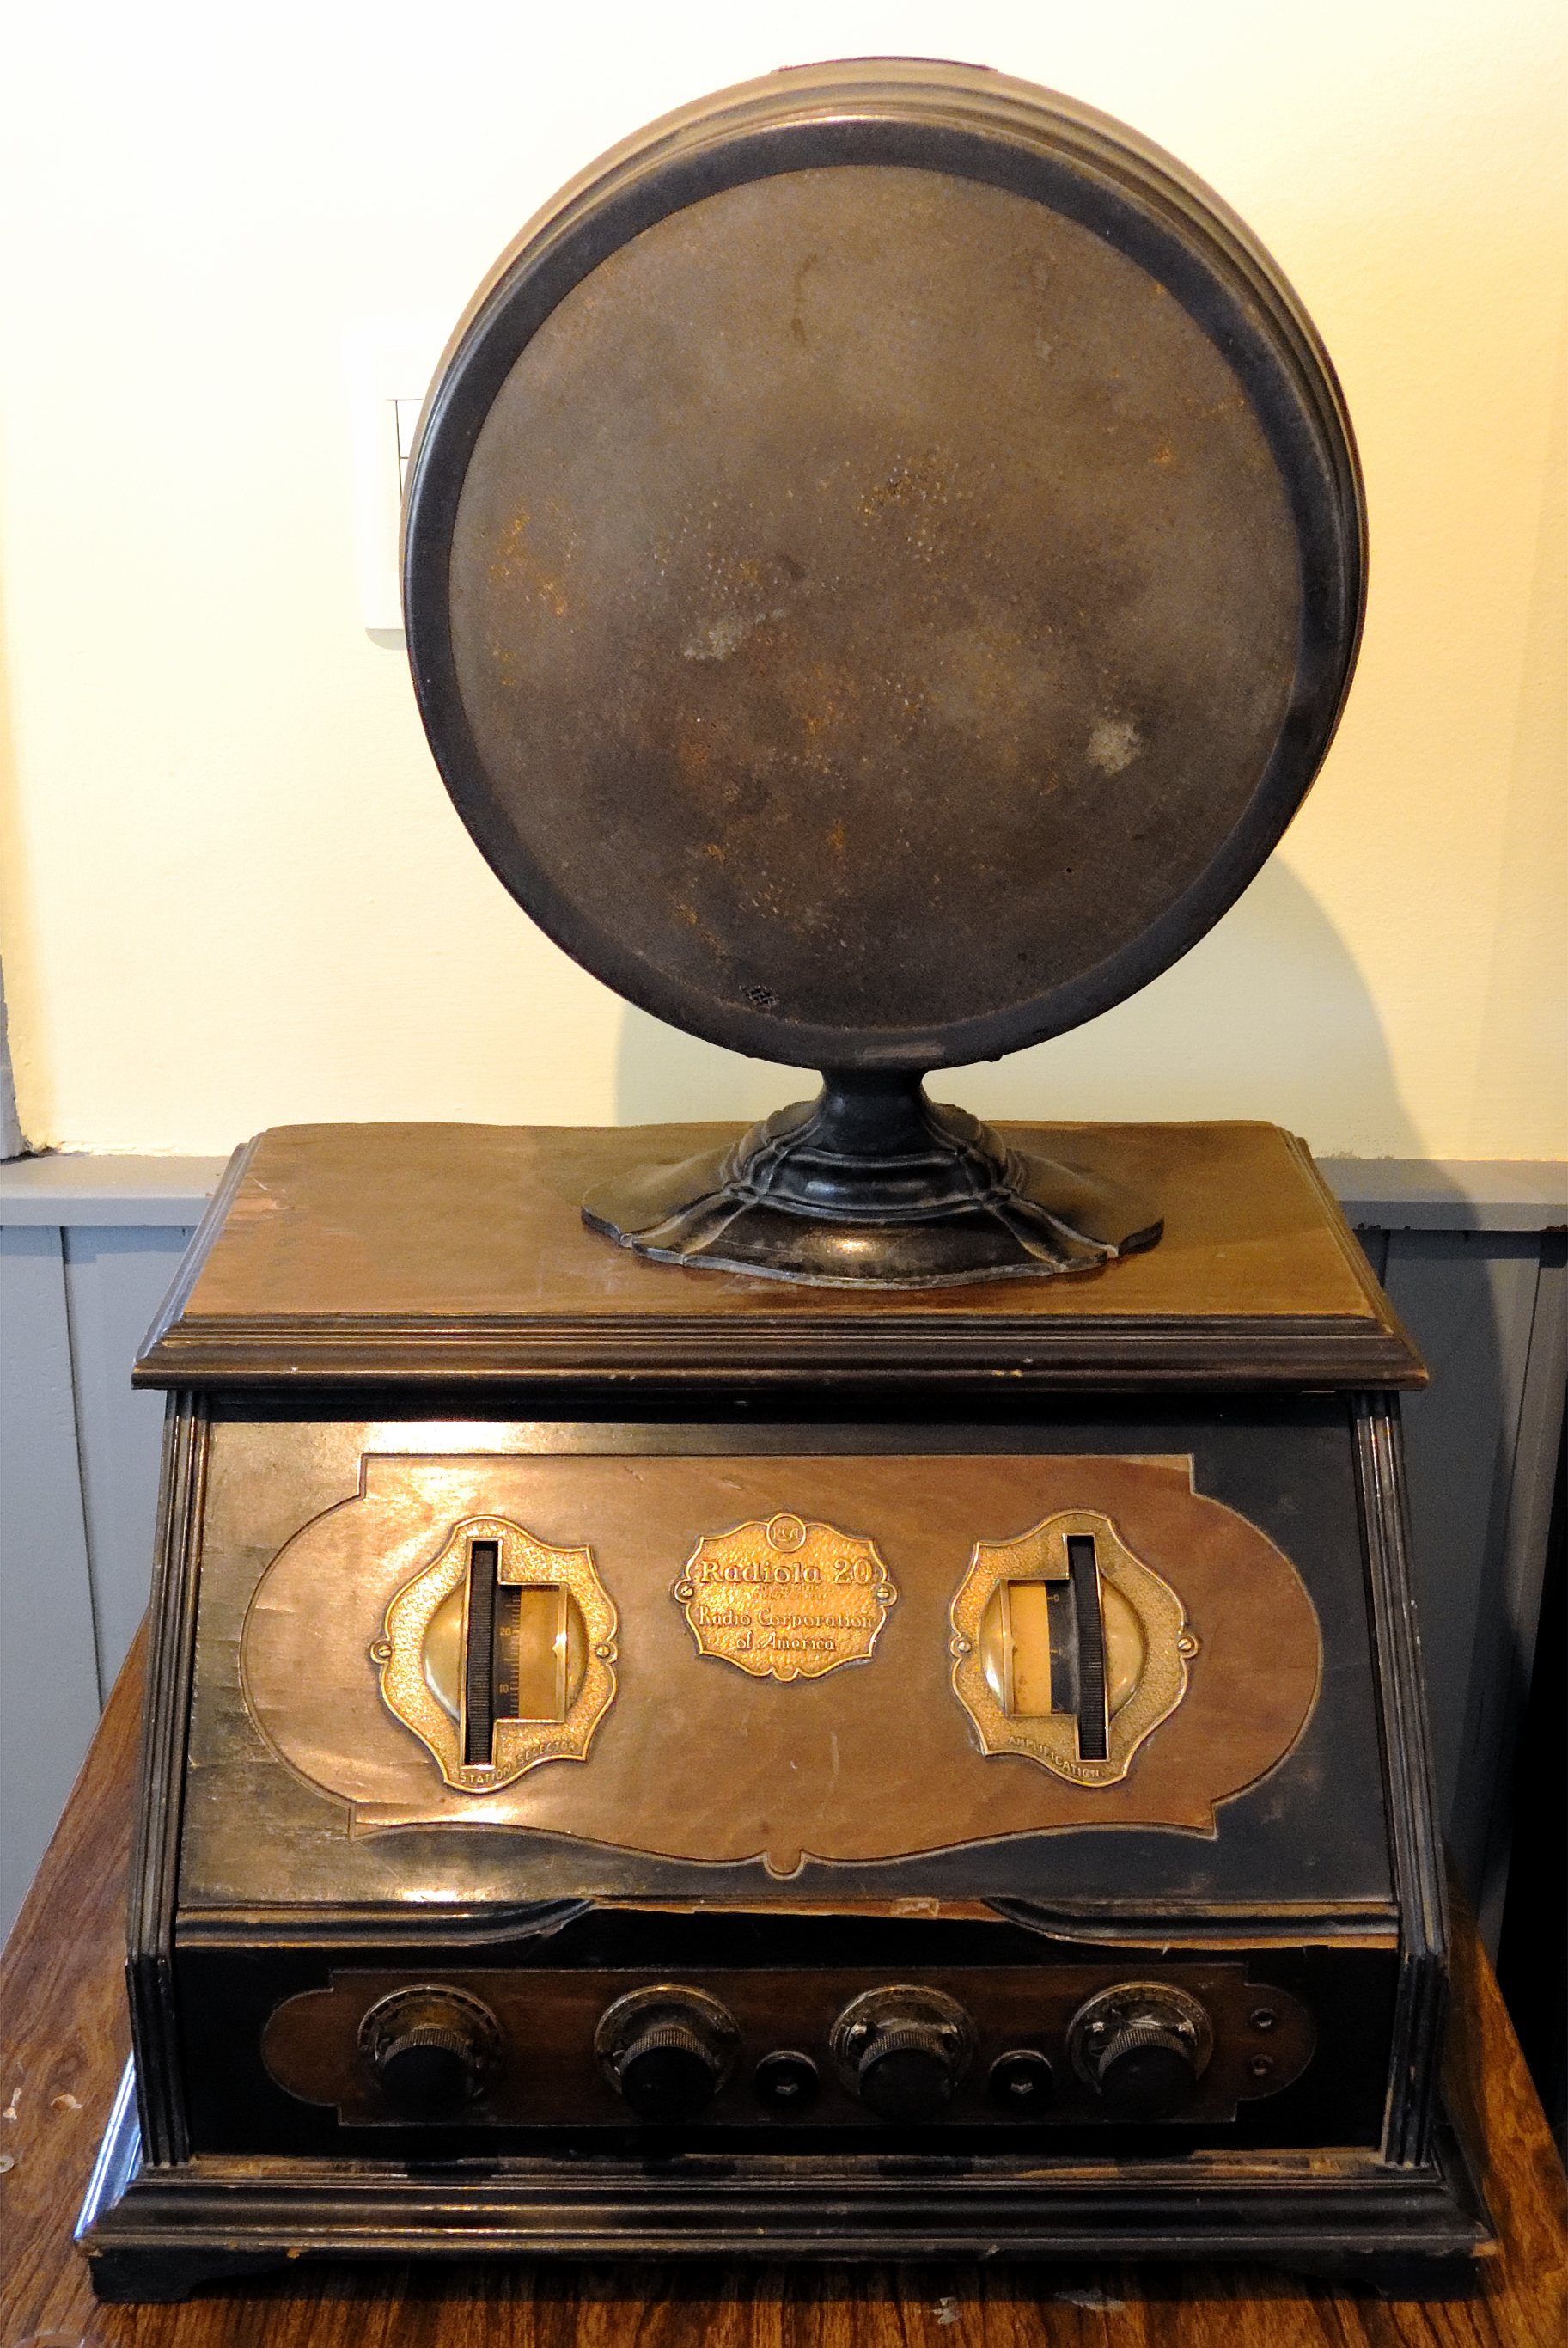
\includegraphics[width=0.55\textwidth]{../figures/early_radio.jpg}
        \caption{Radio primitiva. \cite{wiki:historia_radio}}
      \end{figure}
    \end{column}
  \end{columns}
\end{frame}

\begin{frame}{Aislamiento en Tubos de Vacío}
  \frametitle{Componentes Críticos para Válvulas Termoiónicas}
  Los \textbf{tubos de vacío} fueron el componente activo central de la
  electrónica en la primera mitad del siglo XX.

  \begin{columns}[T]
    \begin{column}{0.6\textwidth}
      \begin{itemize}[<+->]
        \item Las bases de estos dispositivos debían ser excelentes aislantes y
          soportar el calor de operación.
        \item Se fabricaron con \textbf{porcelana} y \textbf{esteatita},
          asegurando el aislamiento y la integridad estructural.
      \end{itemize}
    \end{column}
    \begin{column}{0.4\textwidth}
      \begin{figure}
        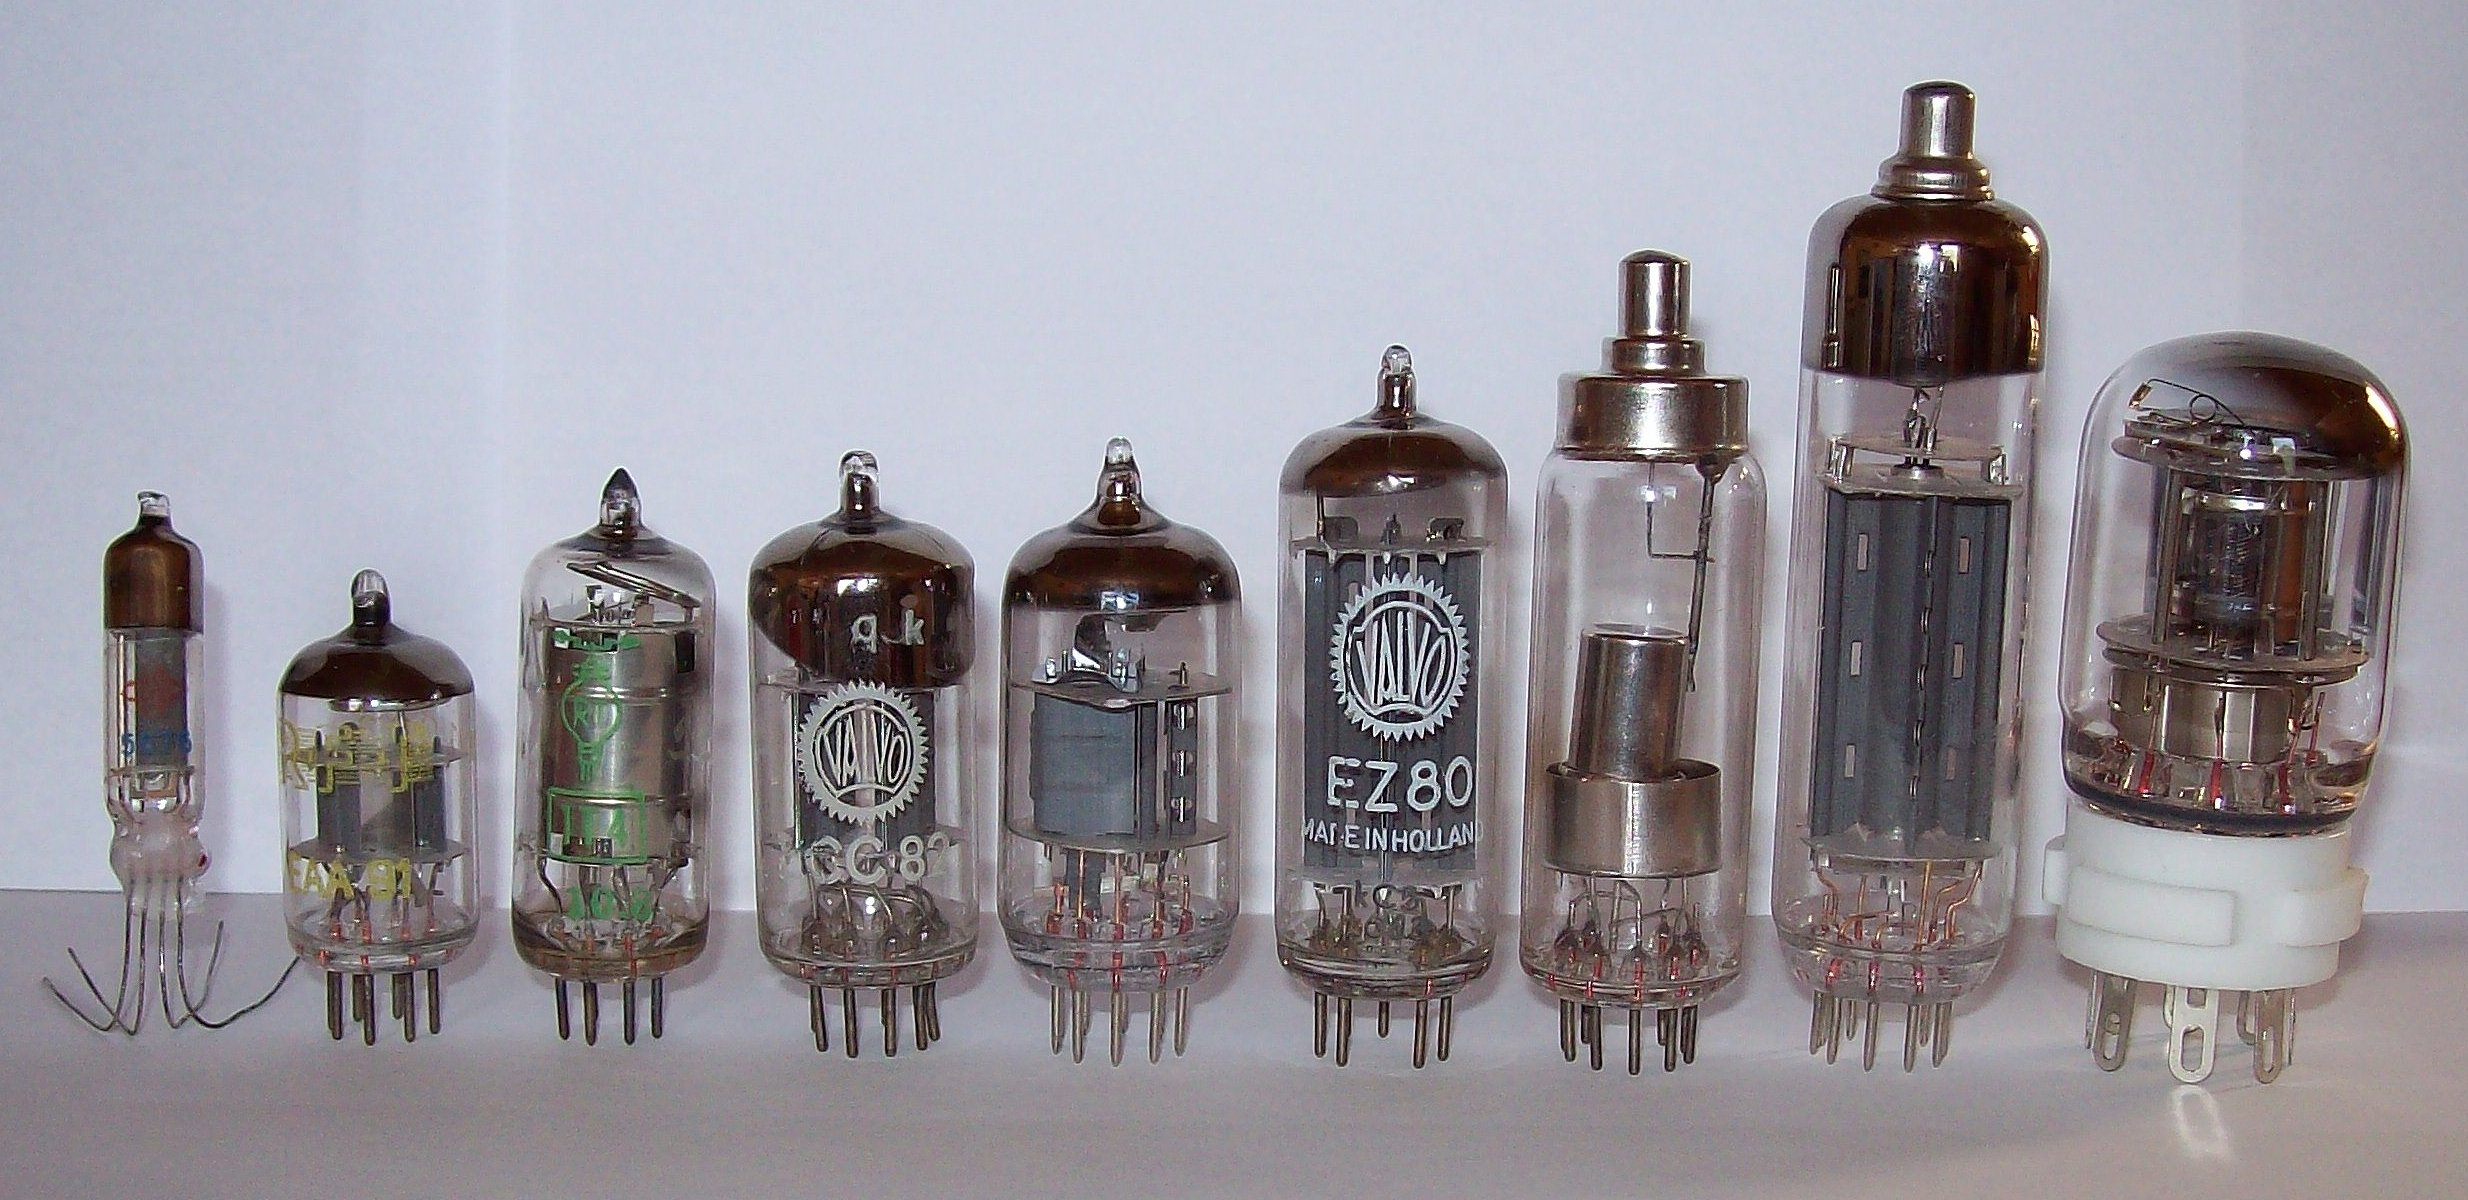
\includegraphics[width=\textwidth]{../figures/vacuum_tubes.jpg}
        \caption{Tubos de vacío. \cite{wiki:vacuum_tube}}
      \end{figure}
    \end{column}
  \end{columns}
\end{frame}

\begin{frame}{Sustratos para Componentes Pasivos}
  \frametitle{Soportes Dieléctricos para Circuitos}
  La construcción de circuitos requería componentes pasivos como resistencias y
  capacitores.

  \begin{columns}[T]
    \begin{column}{0.6\textwidth}
      \begin{itemize}[<+->]
        \item Se utilizaron cerámicos como el \textbf{cuerpo o sustrato
          aislante} de dichos componentes.
        \item El material cerámico proveía el soporte mecánico, el aislamiento
          eléctrico y la disipación de calor.
      \end{itemize}
    \end{column}
    \begin{column}{0.4\textwidth}
      \begin{figure}
        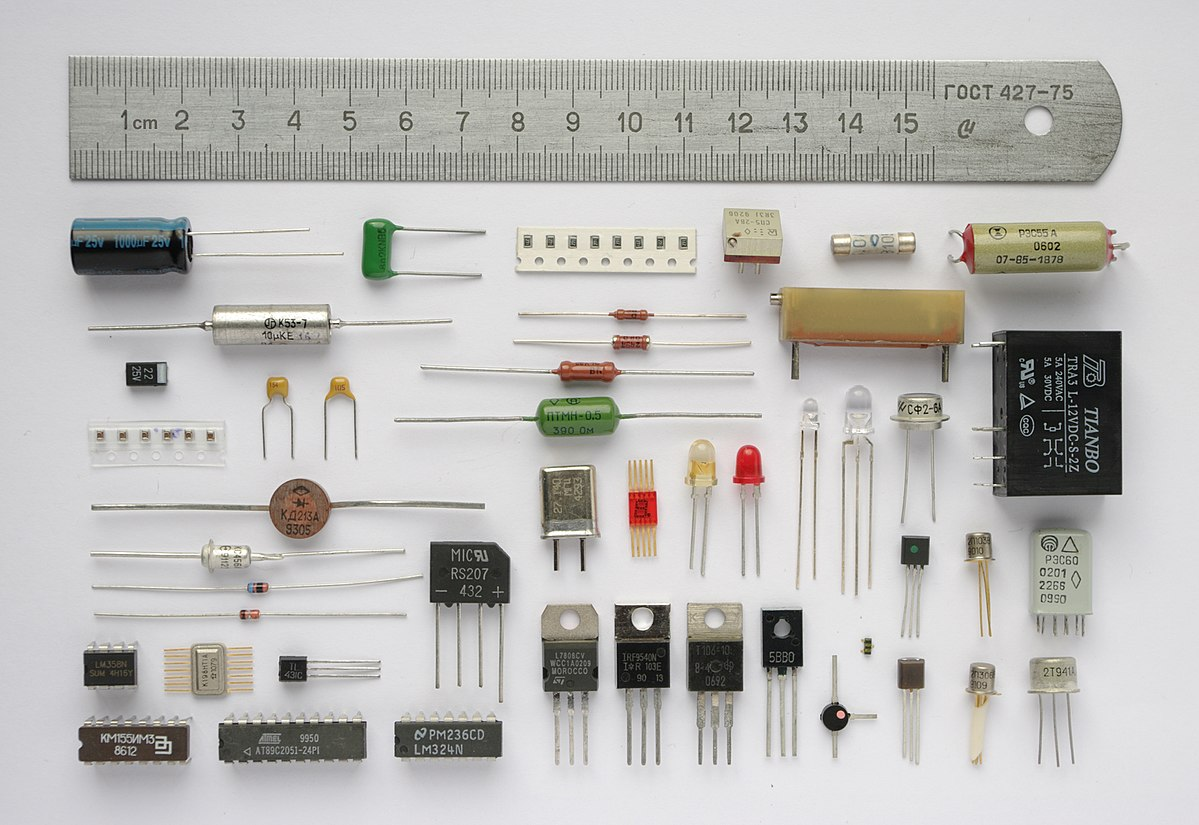
\includegraphics[width=\textwidth]{../figures/passive_components.jpg}
        \caption{Componentes electricos. \cite{wiki:electronic_component}}
      \end{figure}
    \end{column}
  \end{columns}
\end{frame}

\begin{frame}{Puntos importantes}
  \frametitle{Conclusiones}
  \begin{itemize}[<+->]
    \item En el período analizado (1750-1950), la cerámica se consolidó como un
      \textbf{material de ingeniería} indispensable.
    \item Si bien no fue una tecnología principal, funcionó como una
      \textbf{tecnología habilitadora fundamental}.
    \item Sus propiedades refractarias, de inercia química y de aislamiento
      dieléctrico fueron un requisito previo para el desarrollo de la
      siderurgia, la industria química y la electrificación.
  \end{itemize}
\end{frame}
